\section{Servizi e accesso al canale condiviso}
Lo scopo del livello di \textbf{collegamento dati} è la gestione e risoluzione dei problemi associati alla trasmissione sul singolo hop, senza
conoscere l'intera topologia della rete. Offre quindi servizi di: \begin{itemize}
    \item \textbf{Framing}: Molti protocolli di questo livello incapsulano i datagrammi all'interno di un frame prima di trasmetterlo, la cui struttura
    è definita dal primo.
    \item \textbf{Accesso al mezzo condiviso}: È necessario che i protocolli forniscano un \textbf{Medium Access Control} (MAC) per l'accesso ai
    collegamenti, il quale specifica le regole con cui immettere i frame nel socket. Saranno approfonditi nella sezione successiva.
    \item \textbf{Consegna affidabile}: I protocolli che forniscono questo servizio sono utilizzati in un contesto dove è comune trovare errori nella
    trasmissione, ed è quindi necessario implementare una funzione per la relativa gestione.
    \item \textbf{Rilevazione e gestione errori}: Può capitare che a causa di disturbi del segnale i dati vengano corrotti. Per questa ragione, molti
    protocolli forniscono un meccanismo per rilevare questi problemi grazie ad un bit di flag all'interno del frame, il quale sarà controllato dall'host
    ricevente.
\end{itemize}

\noindent I protocolli usati a livello di collegamento dati dipendono dalla tecnologia della porta di rete, come la rete \textbf{Wi-Fi} (IEEE 802.11),
una rete fissa \textbf{Ethernet} (IEEE 802.3), oppure \textbf{Fibra ottica}, che fa uso di Synchronous Digital Hierarchy (SDH) o di Point to Point
Protocol (PPP). È chiaro come questo livello sia strettamente legato all'hardware; infatti il protocollo è realizzato da un \textbf{adattatore di rete}
(scheda di rete), nel quale un chip dedicato ne fornisce i relativi servizi, mentre lato software sono implementate le funzioni per comunicare con i
livelli superiori.\par
Ogni host presenta più interfacce di rete per l'invio e la ricezione dei dati in base alle tecnologia, le quali corrispondono a un collegamento fisico
specifico, definito da un \textbf{Media Access Control Address} (Indirizzo MAC), il quale sarà utilizzato negli header dei protocolli per la scelta del
canale da utilizzare. In quanto condiviso, tuttavia, si presenta il problema di regolamentazione accessi e delimtazione delle trasmissioni. Supponiamo
infatti un router di una rete domestica, al cui access point sono collegati più host, come PC, telefoni, console, etc; questi potrebbero entrare in
contesa se utilizzano i servizi concorrentemente. La soluzione al problema deve cercare al meglio delle sue possibilità di: \begin{itemize}
    \item Minimizzare le collisioni fra le trasmissioni e quindi la perdita di informazioni.
    \item Massimizzare l'utilizzo del mezzo ed evitare sprechi di risorse.
\end{itemize}
\noindent La prima strategia proposta è quella di \textbf{allocazione statica}, la quale vede le risorse suddivise a priori tra i partecipanti. Degli
esempi di questa implementazione sono il Time Division Multiplex (TDM), che divide il tempo in vari slot, ognuno dei quali associato ad ogni utente, e
il Frequency Division Multiplex, che fa lo stesso, ma per le frequenze. La strategia statica non risponde appropriatamente alle nostre richieste,
perché non massimizza l'utilizzo del mezzo; dividendo aprioristicamente le risorse, è inevitabile che quando non ci sia richiesta dagli host, lo slot
ad essi associato sia inutilizzato. Inoltre, con aggiunta o rimozione di altri host sarebbe necessario ricalcolare la divisione delle risorse. La
strategia attualmente in uso è quella di \textbf{allocazione dinamica}, che si divide a sua volta in due tecniche: \begin{itemize}
    \item \textbf{A turno}: Organizzano le stazioni (host) in un determinato ordine e si definisce un token che dona il diritto di trasmissione per un
    determinato intervallo di tempo. Scaduta la disponibilità, si passa all'utente successivo. Questa implementazione in particolare è chiamata
    \textbf{token-ring} e richiede di stabilire un ordine e intervallo di disponibilità del token. Inoltre, più stazioni sono presenti, meno tempo
    potrà essere dedicato alla trasmissione della singola.
    \item \textbf{A contesa}: Non implementano un coordinamento centralizzato e le varie stazioni si contengono l'utilizzo del canale di comunicazione.
    Si tratta della strategia attualmente in uso, della quale studieremo nella prossima sezione i protocolli Aloha, Slotted-Aloha e CSMA.
\end{itemize}

%

\section{Algoritmi di accesso al canale condiviso}
Il primo algoritmo discusso, come anche il più semplice tra tutti, è \textbf{Aloha}. Si tratta di uno schema distribuito che vede più stazioni
indipendenti eseguire la stessa seguente procedura per la trasmissione delle trame. La verifica della collisione avviene tramite "ascolto" del canale.
Viene rilevato un valore di potenza, il quale, se è più alto del normale, indica che stanno già venendo trasmessi dei dati e bisogna attendere il
termine dell'intervallo di tempo calcolato casualmente. Tuttavia, è necessario che le stazioni siano desincronizzate, perché se così non fosse,
continuerebbero a trasmettere le loro trame senza successo. Aloha trova utilizzo ancora oggi grazie alla sua semplicità, per esempio per le chiamate
telefoniche.\par
In uno scenario ideale, Aloha è eseguito in tempo lineare $\Omega(n)$, ma nella realtà è possibile utilizzare al massimo il $19\%$ del suo potenziale.
Definiamo inoltre \textbf{periodo di vulnerabilità} l'intervallo di tempo in cui una trama può subire collisioni, il quale dipende dall'algoritmo usato.
Per quanto riguarda Aloha, ha durata uguale a due volte il tempo di trasmissione usato per la trama. In particolare: \begin{itemize}
    \item \textbf{Tempo di trama}: $T = \text{bitDaTrasmettere} / \text{velocitàTrasmissione}$ 
    \item \textbf{Periodo di vulnerabilità}: $V = 2T$
\end{itemize}
\begin{algorithm}[h]
    \caption{Aloha()}
    \begin{algorithmic}[i]
        \While{Stazione ha dati da trasmettere}
            \State Trasmetti i dati
            \If{Canale è occupato} \Comment{Collisione verificata}
                \State Estrai un tempo casuale da aspettare
            \EndIf
            \While{Tempo non scaduto}
                \State Decrementa il tempo
            \EndWhile
        \EndWhile
    \end{algorithmic}
\end{algorithm}
\begin{figure}[h]
	\centering
	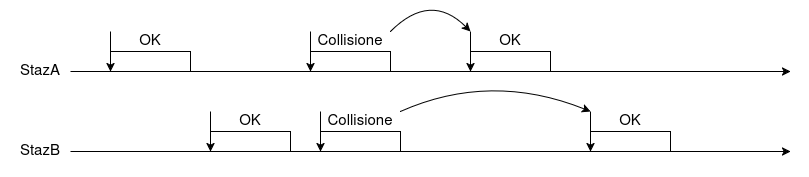
\includegraphics[width=1\linewidth]{Images/aloha.png}
	\caption{Evoluzione di Aloha nel tempo}
\end{figure}

\newpage

\noindent \textbf{Slotted-Aloha} è una versione modificata del precedente algoritmo; suddivide il tempo in vari intervalli di dimensione uguale al
tempo di trama $T$ mantenendo la stessa dinamica di trasmissione senza ascolto del canale, ma permettendola solamente all'inizio di uno di questi
slot.\par
In questo algoritmo una stazione rischia di subire collisioni solo se un'altra sta trasmettendo nello stesso slot, dunque il periodo di
vulnerabilità corrisponde alla grandezza dello slot: il tempo di trama $T$. Ciò si traduce in un'efficienza migliore rispetto all'Aloha base, ovvero
del $38\%$.
\begin{algorithm}[h]
    \caption{slotted-aloha()}
    \begin{algorithmic}[i]
        \While{Stazione ha dati da trasmettere}
            \State Attendi l'inizio dello slot successivo e trasmetti i dati
            \If{Canale è occupato}
                \State Estrai un tempo casuale da aspettare
            \EndIf
            \While{Tempo non scaduto}
                \State Decrementa il tempo
            \EndWhile
        \EndWhile
    \end{algorithmic}
\end{algorithm}
\begin{figure}[h]
	\centering
	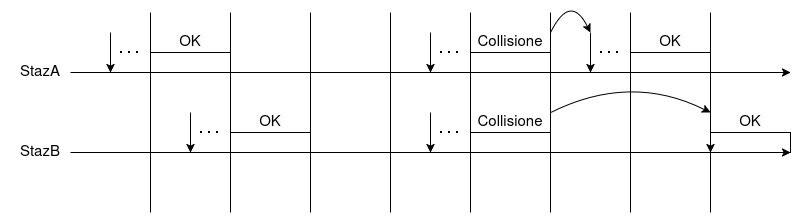
\includegraphics[width=1\linewidth]{Images/slotted_aloha.png}
	\caption{Evoluzione di Slotted-Aloha nel tempo}
\end{figure}

\newpage

\noindent È possibile aumentare ulteriormente l'efficienza riducendo il numero di collisioni con l'algoritmo \textbf{Carrier Sense Multiple Access}
(CSMA) \textbf{persistente}, la prima procedura che continua ad ascoltare il canale fin quando non è libero prima di trasmettere.\par
Sebbene il controllo sulle collisioni possa a primo impatto sembrare superfluo, queste possono avvenire quando due stazioni desiderano
trasmettere una trama e attendono la terminazione di una precedente. Queste inizierebbero la trasmissione allo stesso tempo, collidendo. Per quanto una
gestione migliore del canale rispetto ad Aloha, è per questa ragione, che con un grande numero di stazioni, l'utilizzo del mezzo risulterebbe
estremamente difficile. Si favorirebbero infatti le stazioni con meno latenza, riducendo l'equità generale del mezzo.\par
Si introduce inoltre il \textbf{ritardo di trasmissione} $\tau$, una misura che quantifica il tempo necessario per l'invio del segnale alle altre
stazioni per far sì che leggano il canale occupato. Il segnale non si invia istantaneamente, ed è infatti legato al tempo di vulnerabilità, che in
questo contesto ha generalmente valore $2\tau$.
\begin{algorithm}[h]
    \caption{CSMA-persistent()}
    \begin{algorithmic}[i]
        \While{Stazione ha dati da trasmettere}
            \While{Canale non è libero}
                \State Attendi che si liberi
            \EndWhile
            \State Trasmetti la trama
            \If{Canale è occupato}
                \State Estrai un tempo casuale
            \EndIf
            \While{Tempo non scaduto}
                \State Decrementa il tempo
            \EndWhile
        \EndWhile
    \end{algorithmic}
\end{algorithm}
\begin{figure}[h]
	\centering
	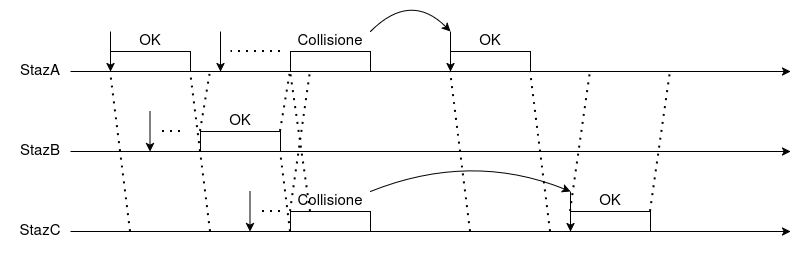
\includegraphics[width=0.8\linewidth]{Images/pers-CSMA.png}
	\caption{Evoluzione di CSMA persistente nel tempo}
\end{figure}

\newpage

\noindent Un altro approccio per cercare di ridurre il numero di collisioni è il \textbf{CSMA non persistente}, una configurazione che non implementa
l'attesa del termine della trasmissione in caso di collisione, bensì solo l'estrazione del tempo da attendere per effetturare un nuovo tentativo, con
lo scopo di aumentare l'equità tra le stazioni. Riduce il numero di collisioni possibili grazie alla generazione di intervalli di attesa casuali.
\begin{algorithm}[h]
    \caption{CSMA-non-persistent()}
    \begin{algorithmic}[i]
        \While{Stazione ha dati da trasmettere}
            \If{Canale è libero}
                \State Trasmetti la trama
            \Else Estrai un tempo casuale
            \EndIf
            \While{Tempo non scaduto}
                \State Decrementa tempo
            \EndWhile
        \EndWhile
    \end{algorithmic}
\end{algorithm}
\begin{figure}[h]
	\centering
	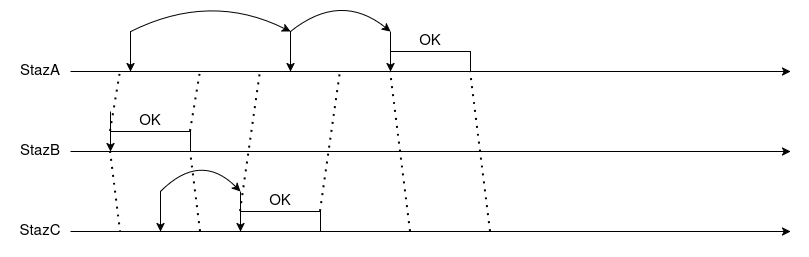
\includegraphics[width=1\linewidth]{Images/nonPersistent_CSMA.png}
	\caption{Evoluzione di CSMA non persistente nel tempo}
\end{figure}

\newpage

\noindent Un ulteriore approccio è fornito dal \textbf{CSMA-p-persistent}, il quale introduce una variabile $p$ configurabile che indica la probabilità
di una stazione di trasmettere la propria trama in un microslot di tempo. Questo implica una riduzione delle collisioni se questi sono stabiliti con una
grandezza sufficiente per tenere conto del ritardo di trasmissione, consentendo una "migliore" lettura del canale. È ugualmente possibile collidere se
due stazioni trasmettono nello stesso microslot, ma è una probabilità molto bassa.
\begin{algorithm}[h]
    \caption{CSMA-p-persistent()}
    \begin{algorithmic}[i]
        \While{Stazione ha dati da trasmettere}
            \If{Canale è libero}
                \State Trasmetti la trama
            \Else
                \While{Canale non è libero}
                    \State Trasmetti la trama con probabilità $p$
                    \State Rimanda la trasmissione di un microslot con probabilità $1-p$
                \EndWhile
            \EndIf
            \If{Collisione verificata}
                \State Estrai un tempo casuale
            \EndIf
            \While{Tempo non scaduto}
                \State Decrementa tempo
            \EndWhile
        \EndWhile
    \end{algorithmic}
\end{algorithm}
\begin{figure}[h]
	\centering
	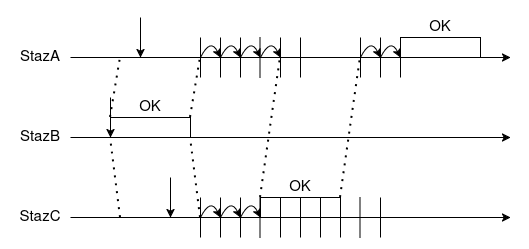
\includegraphics[width=0.7\linewidth]{Images/p-persistent-CSMA.drawio.png}
	\caption{Evoluzione di CSMA P-persistente nel tempo}
\end{figure}

\newpage

\noindent L'ultima sfaccettatura del CSMA, combinabile con tutte le varianti precedenti, è quella di \textbf{Collision Detection} (CSMA-CD), resa
possibile grazie alle nuove architetture, che permette di interrompere la trasmissione in presenza di collisioni. Presentiamo la dinamica applicata
all'algoritmo CSMA persistente.
\begin{algorithm}[h]
    \caption{CSMA-CD()}
    \begin{algorithmic}[i]
        \While{Stazione ha dati da trasmettere}
            \While{Canale non è libero}
                \State Attendi che si liberi
            \EndWhile
            \State Trasmetti la trama
            \If{Canale è occupato}
            \State Interrompi la trasmissione \Comment{Unica aggiunta, sì.}
            \State Estrai un tempo casuale
            \EndIf
            \While{Tempo non scaduto}
                \State Decrementa il tempo
            \EndWhile
        \EndWhile
    \end{algorithmic}
\end{algorithm}
\begin{figure}[h]
	\centering
	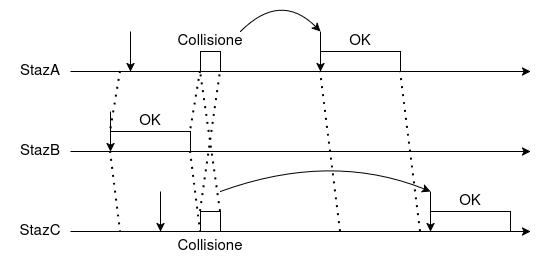
\includegraphics[width=0.7\linewidth]{Images/CD-CSMA.png}
	\caption{Evoluzione di CD-CSMA nel tempo}
\end{figure}

\noindent Grazie alla dinamica di Collision Detection l'efficienza del CSMA aumenta drasticamente, in particolare nel migliore degli scenari fino al
$58\%$ per l'algoritmo persistente, mentre fino al $90\%$ per il p-persistente, con $p = 0.01$.

%

\section{Ethernet, switch e LAN}
Il protocollo \textbf{Ethernet} è quello attualmente più utilizzato nelle reti LAN cablate; si tratta di una tecnologia nata negli anni '70 le cui
prime implementazioni si servivano di un cavo coassiale come bus per connettere ogni nodo. Questa topologia rendeva le reti che ne facevano utilizzo
delle \textbf{LAN Broadcast}, in quanto tutti i frame trasmessi venivano elaborati da tutte le schede di rete connesse al bus.\par
Alla fine degli anni '90 si passa ad una topologia a stella, dove host e router sono collegati direttamente a un \textbf{hub}, un dispositivo a livello
fisico che, ricevuto un bit a un'interfaccia, ne amplifica la potenza e lo trasmette su tutte le altre.\par
Negli anni 2000 Ethernet subì un'altra trasformazione; dove è rimasta la topologia a stella, l'hub è stato sostituito da uno \textbf{switch}, un
apparecchio che svolge funzioni di store-and-forward immune alle collisioni, trasformando le reti in \textbf{Switched LAN}, ovvero reti locali
commutate.\newline

\noindent L'intestazione del protocollo utilizzato, standardizzato da IEEE con codice $802.3$, presenta la seguente struttura: \begin{itemize}
    \item \textbf{Campo dati}: Contiene il datagramma IP la cui dimensione minima dovrà essere $46B$. Se inferiore, si riempie il campo di bit fino a
    raggiungere tale valore, per poi rimuovere lo "stuffing" grazie al campo di lunghezza header del datagramma. Se invece la dimensione supera la MTU di
    $1500B$ il pacchetto dovrà essere frammentato.
    \item \textbf{Indirizzo MAC destinazione}: Indica l'indirizzo hardware della scheda di rete di destinazione. Richiede $6B$.
    \item \textbf{Indirizzo MAC sorgente}: Indica l'indirizzo hardware della scheda di rete di sorgente. Richiede $6B$.
    \item \textbf{Tipo}: Consente a Ethernet di supportare più protocolli di rete. Richiede $2B$.
    \item \textbf{Controllo a ridondanza ciclica}: Svolge una funzione di verifica della correttezza dei bit del frame, equivalente al checksum.
    Richiede $4B$.
    \item \textbf{Preambolo}: Necessario per sincronizzare le stazioni tra di loro grazie ai primi sette byte e a comunicare l'inizio dei dati con gli
    ultimi due bit dell'ultimo byte. In totale richiede $8B$.
\end{itemize}
\begin{figure}[h]
	\centering
	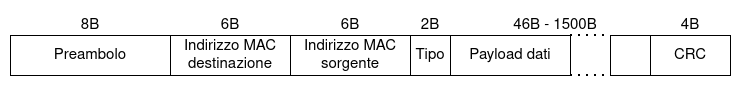
\includegraphics[width=1\linewidth]{Images/header_ethernet.png}
	\caption{Intestazione protocollo Ethernet}
\end{figure}

\noindent 


\begin{comment}
- Come fa un host a conoscere gli indirizzi MAC degli altri host (della propria rete) o del router?
A livello 2 esiste un protocollo Address Resolution Protocol (ARP) che svolge la medesima funzione del DNS, ma per i MAC address. Partendo da un
indirizzo IP, ricava il MAC, per poterlo inserire nel campo adeguato.

(Non entriamo nel formato di ARP, si definisce solo il comportamento)

1. Quando un host non ha un MAC, dato un indirizzo IP, l'host manda in broadcast a livello 2 una richiesta ARP. Questa contiene un campo che segnala
ARP-req e un altro che contiene l'IP per il quale si richiede l'indirizzo hardware. Il pacchetto è incapsulato nell'header L2 con come indirizzo dstMAC
è l'indirizzo IP di destinazione trasmesso in broadcast, mentre srcMAC è il MAC di sorgente.

2. Solo chi possiede l'IP indicato nella richiesta ARP nel campo dstHW, risponde direttamente a chi ha fatto tale richiesta (Se nella stessa lan). Nel
pacchetto ARP di risposta ci sarà l'apposito codice per identificare il tipo di messaggio, c'è l'IP di chi risponde e il suo relativo MAC address in
tre campi diversi. Tutto questo è incapsulato nell'header L2, dove dstMAC corrisponde a quello di chi ha fatto la richiesta e srcMAC è il MAC di chi
sta rispondendo.

Le risposte ARP ottenute vengono memorizzate in una tabella (ARP table, salva anche associazioni tra IP e MAC) in cui ogni entry ha un tempo di
validità, al termine del quale è cancellato.

--- LAN estese
Per lan estese intendiamo degli apparati di livello 2 che sostituiscono il cavo coassiale, il quale storicamente collegava tutti gli host al router
della LAN.
Questi apparati sostitutivi si chiamano switch e sono formati da un insieme di porte alle quali sono collegati i vari host.
Lo switch ha solo il livello di collegamento dati e le varie porte che determinano quello fisico.

Il pacchetto a lv.2 attraversa quindi lo switch dal canale fisico adeguato per essere trasportato al router. Lo switch mantiene una tabella in cui è
associato il MAC address dell'host o del router con la porta alla quale sono connessi.
Per consegna diretta non si passa dal router e lo switch trasmette i pacchetti, mentre per quella indiretta si mette la porta del router, che
decapsulerà il livello di rete e procederà a trasmettere con routing etc.

-- Altre configurazioni
Gli switch si possono collegare tra di loro. Per gestire un edificio con più piani, per esempio, ogni piano avrà il proprio switch che gestirà gli host
del rispettivo piano.
Tuttavia sarà necessario anche usare uno switch radice che avrà interfaccia verso internet (quindi ha il router connesso a una sua porta) e userà le
sue porte per connettersi agli altri switch, consentendo ad ogni host di accedere a internet.

Dal punto di vista dello switch ci sono tutti i mac address che fanno capo allo switch del piano. I messaggi di broadcast sono trasmessi a tutti e dico
tutti gli host della rete, dal punto di vista della radice vede solamente a quale porta rigirare, senza che l'amministratore di rete debba riconfigurare
nulla. Attenzione solo a non creare cicli, perché in tal caso lo switch vedrebbe più porte associate ad uno stesso MAC address.
\end{comment}



%

\section{Wireless LAN}